\documentclass[10pt,fleqn]{article} % Default font size and left-justified equations
\usepackage{import}
\usepackage[%
    pdftitle={Energie et puissance d'un smartphone},
    pdfauthor={Geoffrey Vaquette}]{hyperref}
\subimport{../../../../style/}{preambule}
%\fichetrue
\fichefalse

\proftrue
%\proffalse

\tdtrue
%\tdfalse

\courstrue
%\coursfalse

\subimport{../../../../style/}{new_style}
\subimport{../../../../style/}{macros_SII}
\subimport{../../../../style/}{preambule_trou}

\usepackage{siunitx}
% -------------------------------------
% Déclaration des titres
% -------------------------------------

\def\discipline{Enseignement \\Technologique \\ Transversal}
\def\xxtete{Enseignement Technologique Transversal}

\def\classe{1 STI2D}
\def\xxnumpartie{Séquence 2}
\def\xxpartie{Energie électrique et puissance d'un smartphone}

\def\xxnumchapitre{Séance 3}
\def\xxchapitre{\hspace{.12cm} Énergies, Puissances et rendement}

\def\xxposongletx{2}
\def\xxposonglettext{1.45}
\def\xxposonglety{23}
\def\xxonglet{Seq. 2 -- TD 3}

\def\xxactivite{Synthèse}
\def\xxauteur{\textsl{Geoffrey Vaquette}}

\def\xxcompetences{%
\textsl{%
\textbf{Savoirs et compétences :}
\begin{itemize}[label=\ding{112},font=\color{ocre}]
\item CO2.1	Identifier les flux et la forme de l'énergie, caractériser ses transformations et/ou modulations et estimer l'efficacité globale d'un système.
\end{itemize}
%
}}

\def\xxfigures{
\begin{center}

\end{center}
}%figues de la page de garde
\def\xxpied{%
Chaine d'énergie -- \xxactivite%
}

%---------------------------------------------------------------------------

\renewcommand{\RemplirTrou}{true}
\title{Le bloc « adapter » du robot mbot}
\date{}
\begin{document}
\maketitle
\chapterimage{}
%\pagestyle{empty}


%\chapterentete{}

\iftd
\begin{tikzpicture}[remember picture,overlay]
\node at (current page.north west)
{\begin{tikzpicture}[remember picture,overlay]
\draw[anchor=west] (-2cm,-3.25cm) node [line width=2pt,rounded corners=15pt,draw=ocre,fill=white,fill opacity=0.6,inner sep=40pt]{\strut\makebox[22cm]{}};
\draw[anchor=west] (1cm,-3.25cm) node {\huge\sffamily\bfseries\color{black} %
\begin{minipage}{1cm}
\rotatebox{90}{\LARGE\sffamily\textsc{\color{ocre}\textbf{\xxnumpartie}}}
\end{minipage} \hfill
\begin{minipage}[c]{13.5cm}
\begin{titrepartie}
\begin{flushright}
\renewcommand{\baselinestretch}{1.1} 
\Large\sffamily\textsc{\textbf{\xxpartie}}
\renewcommand{\baselinestretch}{1} 
\end{flushright}
\end{titrepartie}
\end{minipage} \hfill
\begin{minipage}[c]{3.5cm}
{\large\sffamily\textsc{\textbf{\color{ocre} \discipline}}}
\end{minipage} 
 };
\end{tikzpicture}};
\end{tikzpicture}


\else
\begin{tikzpicture}[remember picture,overlay]
\node at (current page.north west)
{\begin{tikzpicture}[remember picture,overlay]
\node[anchor=north west,inner sep=0pt] at (0,0) {\includegraphics[width=\paperwidth, height=5cm]{\thechapterimage}};
\draw[anchor=west] (-2cm,-8cm) node [line width=2pt,rounded corners=15pt,draw=ocre,fill=white,fill opacity=0.6,inner sep=40pt]{\strut\makebox[22cm]{}};
\draw[anchor=west] (1cm,-8cm) node {\huge\sffamily\bfseries\color{black} %
\begin{minipage}{1cm}
\rotatebox{90}{\LARGE\sffamily\textsc{\color{ocre}\textbf{\xxnumpartie}}}
\end{minipage} \hfill
\begin{minipage}[c]{14cm}
\begin{titrepartie}
\begin{flushright}
\renewcommand{\baselinestretch}{1.1} 
\Large\sffamily\textsc{\textbf{\xxpartie}}
\renewcommand{\baselinestretch}{1} 
\end{flushright}
\end{titrepartie}
\end{minipage} \hfill
\begin{minipage}[c]{3.5cm}
{\large\sffamily\textsc{\textbf{\color{ocre} \discipline}}}
\end{minipage} 
 };
\end{tikzpicture}};
\end{tikzpicture}

\fi



% Chapitre + TABLE DES MATIERES(dans le cas du cours)
\iftd
\vfill
\begin{tikzpicture}[overlay]
\node[shape=rectangle, 
      rounded corners = .25 cm,
	  draw= ocre,
	  line width=2pt, 
	  fill = ocre!10,
	  minimum width  = 2.5cm,
	  minimum height = 3cm,] at (18cm,0) {};
\node at (17.7cm,0) {\rotatebox{90}{\textbf{\Large\color{ocre}{\classe}}}};
%{};
\end{tikzpicture}

\vspace {3.5 cm}

\begin{tikzpicture}[remember picture,overlay]
\draw[anchor=west] (-2cm,-6cm) node {\huge\sffamily\bfseries\color{black} %
\begin{minipage}{2cm}
\LARGE\sffamily\textsc{\color{ocre}\textbf{\xxactivite}}
\end{minipage} \hfill
\begin{minipage}[c]{15cm}
\begin{titrechapitre}
\renewcommand{\baselinestretch}{1.1} 
\Large\sffamily\textsc{\textbf{\xxnumchapitre}}

\Large\sffamily\textsc{\textbf{\xxchapitre}}
\vspace{.5cm}

\renewcommand{\baselinestretch}{1} 
\normalsize\normalfont
\xxcompetences
\end{titrechapitre}
\end{minipage}  };
\end{tikzpicture}

\else


\begin{tikzpicture}[overlay]
\node[shape=rectangle, 
      rounded corners = .25 cm,
	  draw= ocre,
	  line width=2pt, 
	  fill = ocre!10,
	  minimum width  = 2.5cm,
	  minimum height = 3cm,] at (18cm,0) {};
\node at (17.7cm,0) {\rotatebox{90}{\textbf{\Large\color{ocre}{\classe}}}};
%{};
\end{tikzpicture}

\vspace{3.5cm}

\begin{tikzpicture}[remember picture,overlay]
\draw[anchor=west] (-2cm,-6cm) node {\huge\sffamily\bfseries\color{black} %
\begin{minipage}{2cm}
\LARGE\sffamily\textsc{\color{ocre}\textbf{\xxactivite}}
\end{minipage} \hfill
\begin{minipage}[c]{15cm}
\begin{titrechapitre}
\renewcommand{\baselinestretch}{1.1} 
\Large\sffamily\textsc{\textbf{\xxnumchapitre}}

\Large\sffamily\textsc{\textbf{\xxchapitre}}
\vspace{.5cm}

\renewcommand{\baselinestretch}{1} 
\normalsize\normalfont
\xxcompetences
\end{titrechapitre}
\end{minipage}  };
\end{tikzpicture}
\vfill

\begin{flushright}
\begin{minipage}[c]{.3\linewidth}
\begin{center}
\xxfigures
\end{center}
\end{minipage}\hfill
\begin{minipage}[c]{.6\linewidth}
\startcontents
\printcontents{}{1}{}
\end{minipage}
\end{flushright}

\begin{tikzpicture}[remember picture,overlay]
\draw[anchor=west] (4.5cm,-.7cm) node {
\begin{minipage}[c]{.2\linewidth}
\begin{flushright}

\includegraphics[width=2cm]{../png/logoCC}
\end{flushright}
\end{minipage}
\begin{minipage}[c]{.2\linewidth}
\textsl{\xxauteur} \\
\textsl{\classe}
\end{minipage}
 };
\end{tikzpicture}
\newpage
\pagestyle{fancy}
\fi
\begin{obj}
  On propose dans cette activité de caractériser le fonctionnement d'un pont en H en vue d'alimenter les moteurs du robot \textit{mbot}
\end{obj}
\section{Introduction}
Soit le montage suivant :
  \begin{center}
    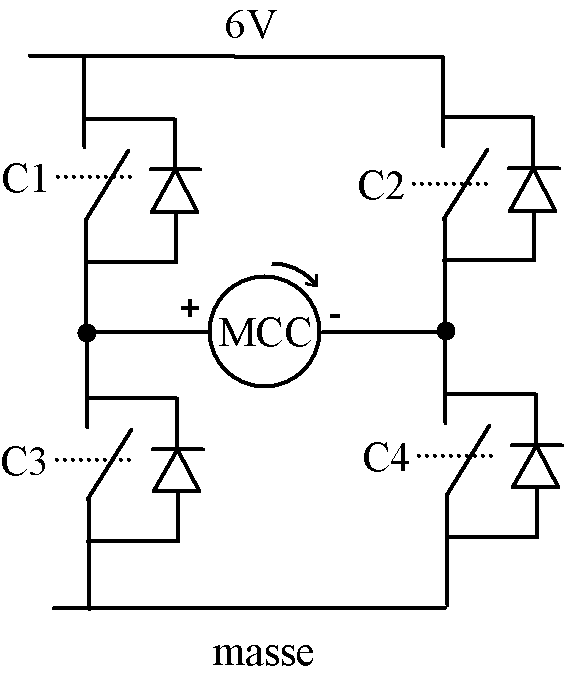
\includegraphics[height=.25\textheight]{images/pontH}
  \end{center}
  Le moteur est commandé par 4 interrupteurs (C1, C2, C3 et C4)

  Rappel sur le fonctionnement d’un Mcc :
\begin{itemize}
  \item Lorsque le moteur est alimenté normalement, c’est à dire lorsque le 6V est sur le + et la masse (0V) sur le -, le moteur tourne dans le sens indiqué.
  \item Si on inverse, c’est à dire si la masse est sur le + et le 6V sur le -, le moteur tourne dans l’autre sens.
\end{itemize}
\begin{question}
  Quels interrupteurs doit-on fermer pour que le moteur tourne dans le sens indiqué ?
\end{question}
\vspace{\stretch{1}}
\begin{question}
  Faites le schéma équivalent en remplaçant les interrupteurs par leur schéma équivalent (un fil quand il est fermé, rien, c’est à dire qu’on l’enlève, quand il est ouvert).
\end{question}
\vspace{\stretch{3}}
\pagebreak
\begin{question}
Quels interrupteurs doit-on fermer pour que le moteur tourne dans le sens inverse ?
\end{question}
    \vspace{\stretch{1}}
\begin{question}
   Faites le schéma équivalent en remplaçant les interrupteurs par leur schéma équivalent (un fil quand il est fermé, rien quand il est ouvert).
\end{question}
    \vspace{\stretch{3}}

    Le schéma réel est le suivant :
    \begin{center}
      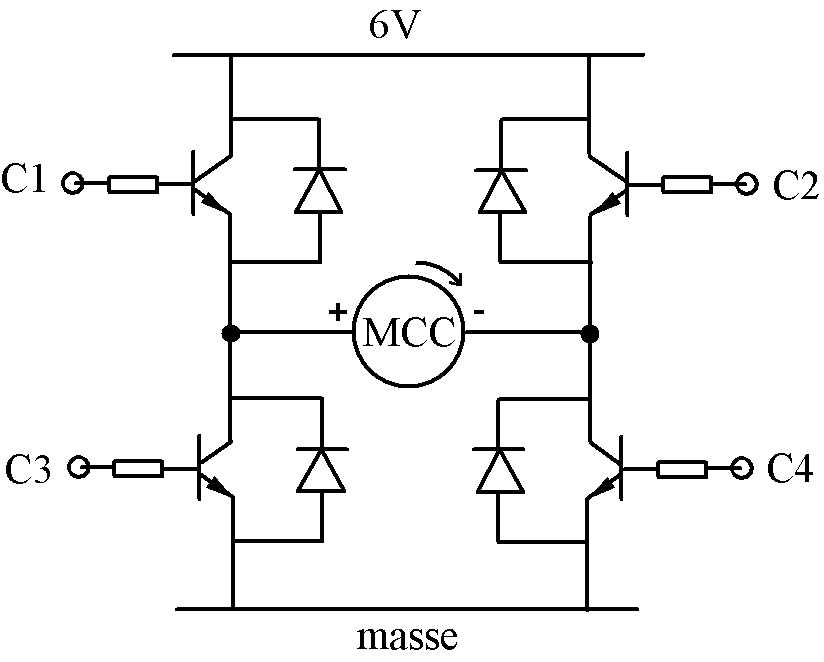
\includegraphics[height=.23\textheight]{images/Pont_en_H3}
    \end{center}
    \begin{question}
      Placez sur chaque transistor les borne E, B et C et rappelez leur noms complet
    \end{question}
    \vspace{\stretch{1}}
    \begin{question}
      Rappelez l'équation liant $I_B$ et $I_C$
    \end{question}
    \vspace{\stretch{1}}
    \begin{question}
      En considérant que $\beta=100$ et un courant dans le moteur $I_M=\SI{0.66}{A}$, calculez le courant $I_B$ pour que le transistor soit saturé (coefficient de sursaturation de 2).
    \end{question}
    \vspace{\stretch{2}}
\end{document}
